\documentclass[11pt]{article}
\usepackage{graphicx}
\usepackage{epstopdf} 
\begin{document}
\begin{titlepage}
%\selectlanguage{english}

%----------------------------------------------------------------------------------------
% TITLE PAGE INFORMATION
%----------------------------------------------------------------------------------------
  \begin{center} % Center everything on the page

  %----------------------------------------------------------------------------------------
  % HEADING SECTIONS
  %----------------------------------------------------------------------------------------
  \textsc{\large Facultatea Calculatoare, Informatica si Microelectronica}\\[0.5cm]
  \textsc{\large Universitatea Tehnica a Moldovei}\\[1.2cm] % Name of your university/college
  \vspace{25 mm}

  \textsc{\Large Medii Interactive de Dezvoltare a Produselor Soft}\\[0.5cm] % Major heading such as course name
  \textsc{\large Lucrarea de laborator\#1}\\[0.5cm] % Minor heading such as course title
  %\textsc{\large Laboratory work}\\[0.5cm] % Minor heading such as course title

\newcommand{\HRule}{\rule{\linewidth}{0.5mm}} % Defines a new command for the horizontal lines, change thickness here

  %----------------------------------------------------------------------------------------
  % TITLE SECTION
  %----------------------------------------------------------------------------------------
  \vspace{10 mm}
  \HRule \\[0.4cm]
  { \LARGE \bfseries Version Control Systems si modul de setare a unui server  }\\[0.4cm] % Title of your document
  \HRule \\[1.5cm]

  %----------------------------------------------------------------------------------------
  % AUTHOR SECTION
  %----------------------------------------------------------------------------------------
      \vspace{30mm}

      \begin{minipage}{0.4\textwidth}
      \begin{flushleft} \large
      \emph{Autor:}\\
      Cristina \textsc{Bradu}
      \end{flushleft}
      \end{minipage}
      ~
      \begin{minipage}{0.4\textwidth}
      \begin{flushright} \large
      \emph{lector asistent:} \\
      Irina \textsc{Cojanu} \\ % Supervisor's Name 
      \emph{lector superior:} \\
      Radu \textsc{Melnic} % Supervisor's Name
      \end{flushright}
      \end{minipage}\\[4cm]

      \vspace{5 mm}
      % If you don't want a supervisor, uncomment the two lines below and remove the section above
      %\Large \emph{Author:}\\
      %John \textsc{Smith}\\[3cm] % Your name

      %----------------------------------------------------------------------------------------
      % DATE SECTION
      %----------------------------------------------------------------------------------------

      %{\large \today}\\[3cm] % Date, change the \today to a set date if you want to be precise

      %----------------------------------------------------------------------------------------
      % LOGO SECTION
      %----------------------------------------------------------------------------------------

      %\includegraphics{red}\\[0.5cm] % Include a department/university logo - this will require the graphicx package

      %----------------------------------------------------------------------------------------

      \vfill % Fill the rest of the page with whitespace
      \end{center}
      
\end{titlepage}

\begin{LARGE}
\textit{Lucrarea de laborator nr.1}
\end{LARGE}

\section{Scopul lucrarii de laborator}

De a se invata utilizarea unui Version Control System si modul de setare a
unui server.

\section{Obiective}

Studierea Version Control Systems (git).

\section{Analiza lucrarii de laborator}

\subsection{Cerintele implementate}

Initializarea unui nou repozitoriu.

Configurarea VCS.

Commit, Push pe branch.

Folosirea fisierului .gitignore.

Revenire la versiunele anterioare.

Crearea branch-urilor noi.

Commit pe ambele branch-uri.

Merge la 2 branchuri.

Rezolvarea conflictelor.


\subsection{Continutul lucrarii}
Link-ul repozitoriului: 
\begin{center}
\textbf{https://github.com/BraduCristina/MIDPS}
\end{center}

Pentru a incepe lucrul cu git-ul, am configurat
\\numele utilizatorului pe github.com si e-mail-ul meu,
\\utilizind comenzile date de figure 1.

In mod scris, acestea arata astfel:
\begin{center}
\textbf{git config --global user.name "NumeUtilizator"}

\textbf{git config --global user.email "email@mail.ru"}
\end{center}

Pentru a configura numele si e-mailul, facem urmatorii pasi:
\\Scriem urmatoarele comenzi: (figure 2)

\textbf{git config –global user.name "NUMELE"}

\textbf{git config –global user.email EMAIL}

\textbf{git config --list} afiseaza e-mail-ul si 
numele utilizatorului(figure 3).

\textbf{git help commit} ofera ajutor in lucrul cu git.
\\Analog este \textbf{git commit -help} (figure 4).

\textbf{git status} arata statutul 
\\repozitoriului nostru.
\\Initial, pentru apelarea acestuia, este necesara
indicarea mapei in care se afla fisierele noastre.

\textbf{cd numemapa}.
In cazul nostru vom folosi instructiunea din figure 5.

\textit{cd MIDPS}

Pentru a lucra cu fisierul .gitignore, initializam fisierele
\textit{README.md} si un \textit{.gitignore}. Fisierul README.md il completam
cu ceva informatie care dorim sa fie afisata, iar 
in fisierul .gitignore adaugam toate fisierele ce trebuie ignorate. (figure 6)

Fisierele noi create le incarcam pe repozitoriul nopstru.
Pentru aceasta vom avea nevoie de urmatoarele comenzi : 
(figure 7)

\textbf{git add .} - comanda indexeaza toate fisierele.

\textbf{git commit -m "some text"} - facem snapshot la comenzi.

\textbf{git push}- incarcam fisierele indexate pe git.

Pentru asigurarea corectitudinii pasilor facuti,
\\utilizam comenzile din figure 8 si figure 9.

\textbf{git status}

\textbf{git show}

Una dintre caracteristicele principale ale unui VCS este faptul ca ne
\\permite sa revenim la o versiune mai veche. 
\\Aceasta poate fi efectuata cu ajutorul comenzii (figure 10)
\textbf{git reset –TYPE "codul commitului" }
\\Exista diferenta intre –soft si –hard , cind facem soft reset, 
indexurile ramin neschimbate.
\\Iar in cazul cind facem hard reset, pierdem indexurile.


Am creat un fisier nou \textit{revert.txt} in versiunea 1. Dupa care l-am
\\sters si am facut commit la versiunea 2, in care am sters 
fisierul revert.txt si dorim sa revenim la versiunea1. 
La inceput vom lansa comanda 

\textbf{git –log}

care ne arata logul de commituri si codul pentru fiecare commit. 
Pentru aceasta preluam primele 8 cifre de la commit-ul anterior(figure 11)

VCS ne permite sa avem mai multe branch-uri(ramuri).
\\Branch-urile sunt utilizate mai des la lucrul in echipa sau cind
\\lucram paralel la un proiect si apoi dorim sa unim toate modificarile.
(figure 12)

\textbf{git branch "name"} - creeaza un branch nou cu numele "name".

\textbf{git branch} - vizualizarea branchurilor (* indica branchul curent).

\textbf{git branch -d "nume"} - sterge branchul "nume".

\textbf{git checkout -b "name"} - creeaza un branch nou cu numele "name" si face
switch la el.

\textbf{git checkout "nume"} - face switch la branchul "nume".

Comenzi noi:
\\Operarea cu ele e prezentata in figure 13.

\textbf{git branch -u upstream/name} - face track la branchul indicat din 
branchul curent.

\textbf{git branch -u upstream/name "nume"} - face track din branchul
"nume" la branch-ul indicat.

\textbf{git branch –track "name" upstream/name} - creeaza branch-ul "name"
si ii face track la branch-ul indicat.

\textbf{git branch –unset-usptream} - scoate tracking-ul la branch-ul in 
care ne aflam. 
\\(figure 13)

Putem avea conflicte in cazul cind dorim sa facem merge la 2 branchuri
si unele rinduri sunt diferite. In asa caz ne vine in ajutor un mergetool.
\\Drept mergetool am ales \textit{kdiff3}. Pentru a seta kdiff3 ca mergetool 
default, folosim comanda:

\textbf{git config –global merge.tool kdiff3}

In continuare vom lucra cu 2 branchuri - "master" si "new".
\\Vom crea in fiecare branch cite un fisier \textit{"tomerge"},
continutul caruia va fi diferit.(figure 14)

In continuare vom incerca sa facem merge si sa 
\\rezolvam acest conflict. (figure 15)

%--------------------------------------------------
\section{Anexa 1 (figures)}
%--------------------------------------------------
\begin{figure}[h]

\includegraphics{images/1.eps}
\caption{Configurare nume/email}
\end{figure}

\begin{figure}[h]

\includegraphics{images/5.eps}
\caption{Afisarea desfasurata a datelor utilizatorului}
\end{figure}

\begin{figure}[h]
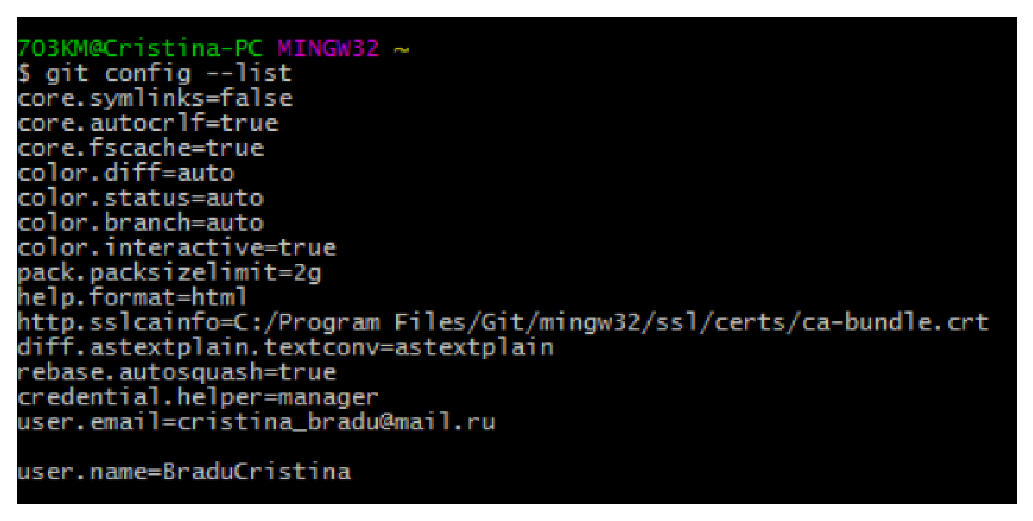
\includegraphics{images/2.eps}
\caption{Afisarea datelor utilizatorului}
\end{figure}

\begin{figure}[h]
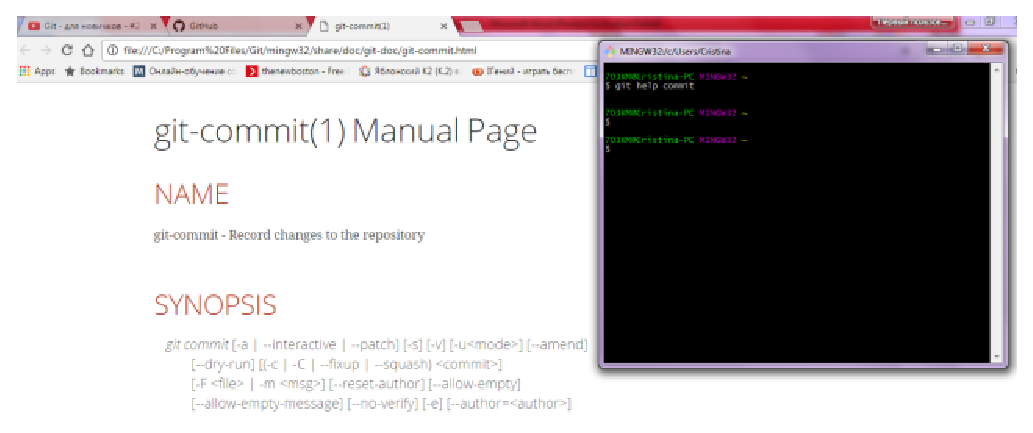
\includegraphics{images/3.eps}
\caption{Ajutor in lucrul cu git}
\end{figure}

\begin{figure}[h]
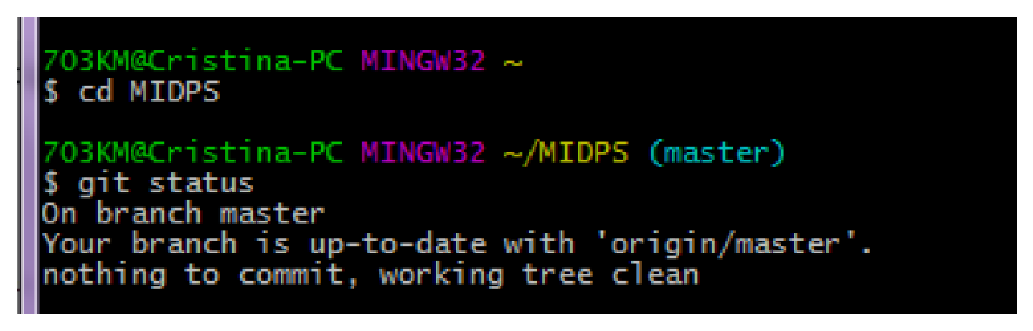
\includegraphics{images/4.eps}
\caption{Afisarea statutului repozitoriului}
\end{figure}

\begin{figure}[h]
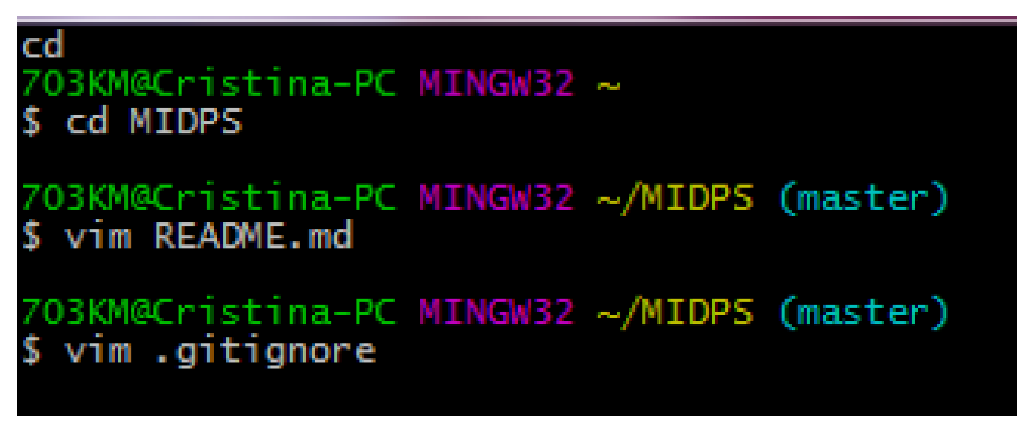
\includegraphics{images/6.eps}
\caption{Adaugarea fisierelor .gitignore si README.md}
\end{figure}

\begin{figure}[h]
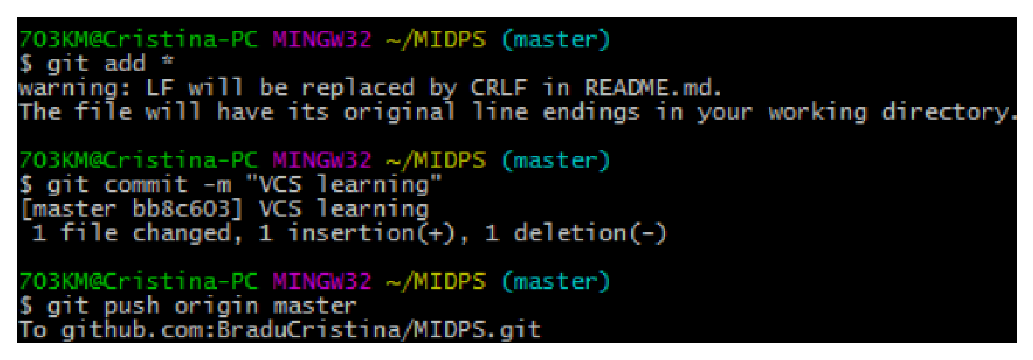
\includegraphics{images/7.eps}
\caption{Adaugarea fisierelor pe github.com}
\end{figure}

\begin{figure}[h]
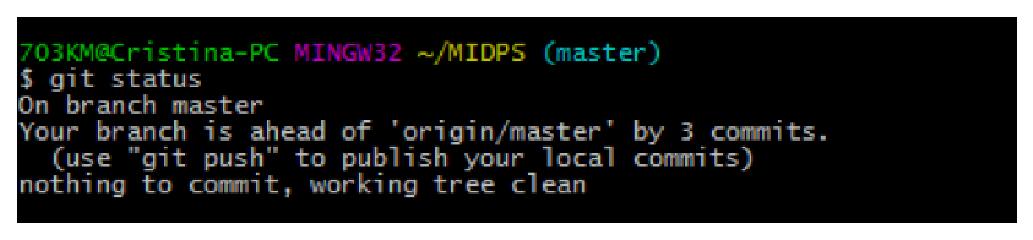
\includegraphics{images/8.eps}
\caption{Verificarea corectitudinii pasilor}
\end{figure}

\begin{figure}[h]
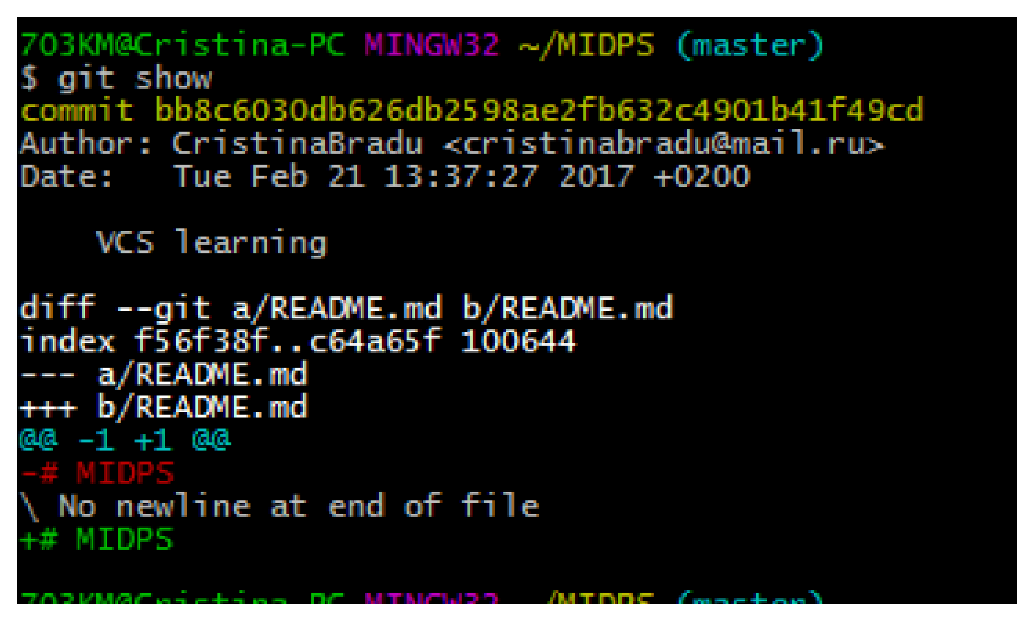
\includegraphics{images/9.eps}
\caption{Verificarea corectitudinii pasilor implementati}
\end{figure}

\begin{figure}[h]
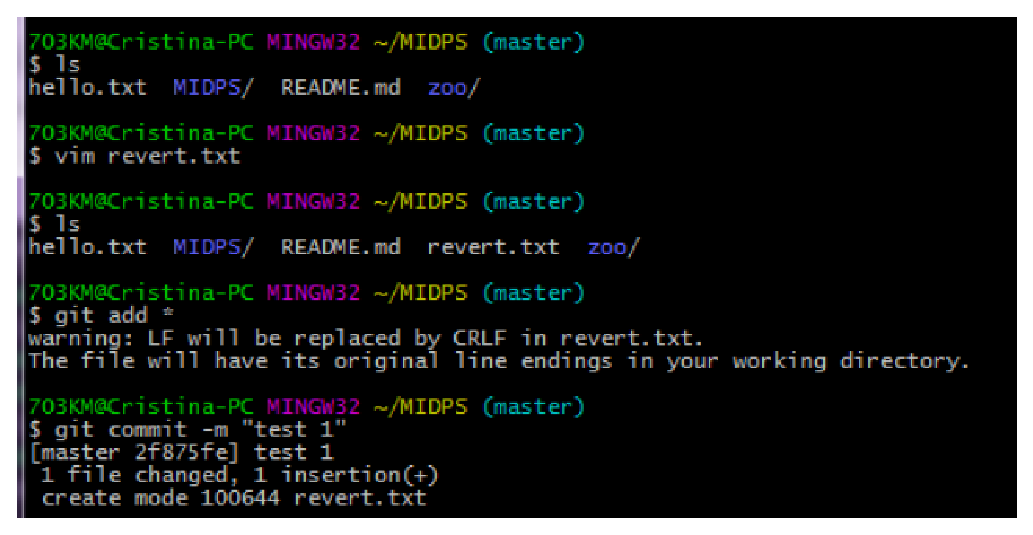
\includegraphics{images/10.eps}
\end{figure}

\begin{figure}[h]
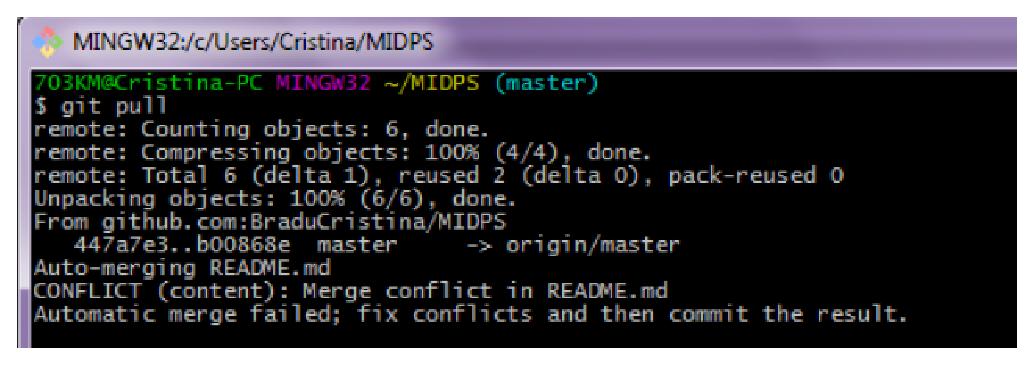
\includegraphics{images/11.eps}
\end{figure}

\begin{figure}[h]

\includegraphics{images/12.eps}
\end{figure}

\begin{figure}[h]
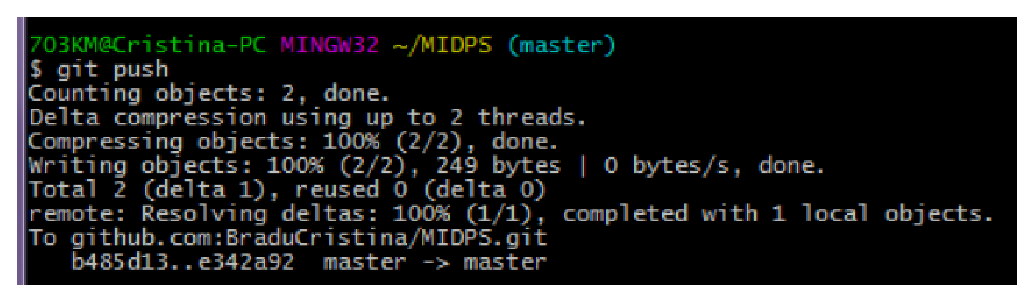
\includegraphics{images/13.eps}
\caption{Revenirea la o versiune mai veche}
\end{figure}

\begin{figure}[h]
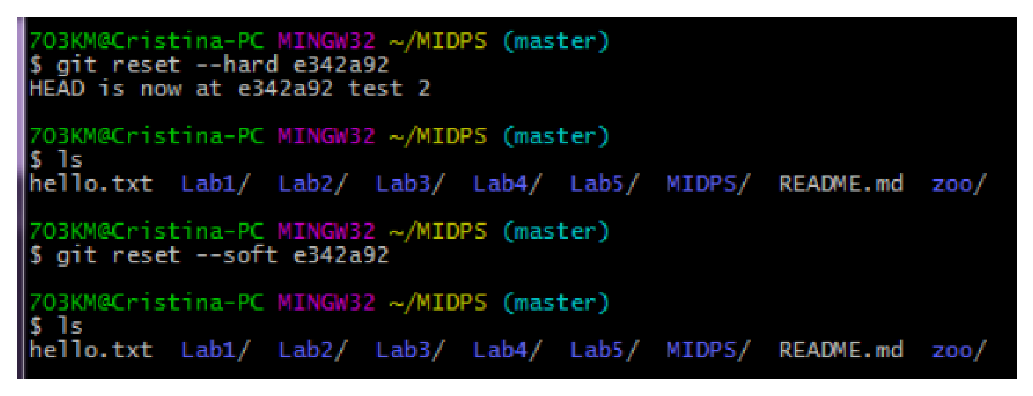
\includegraphics{images/14.eps}
\caption{Log-ul de commit-uri}
\end{figure}

\begin{figure}[h]
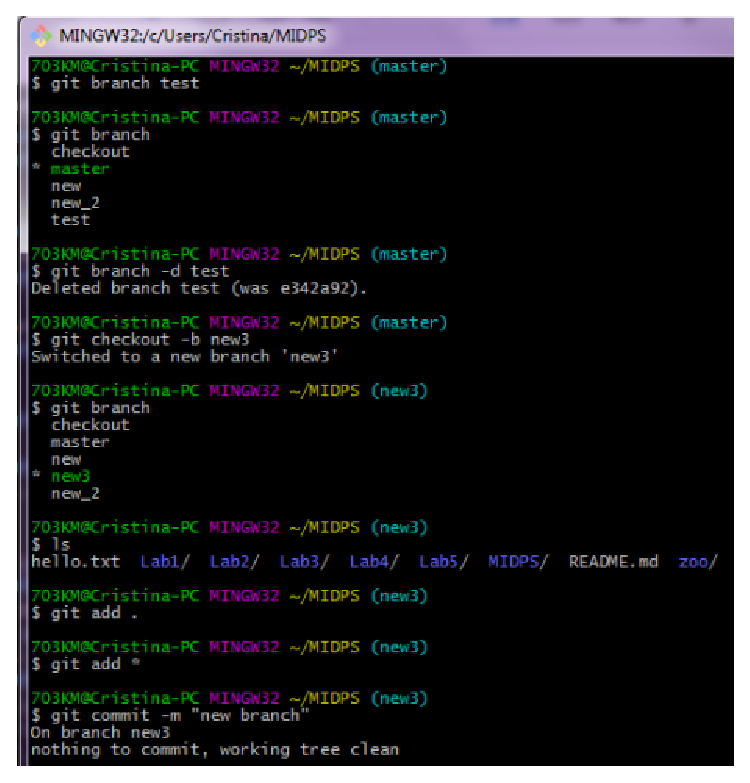
\includegraphics{images/15.eps}
\end{figure}

\begin{figure}[h]
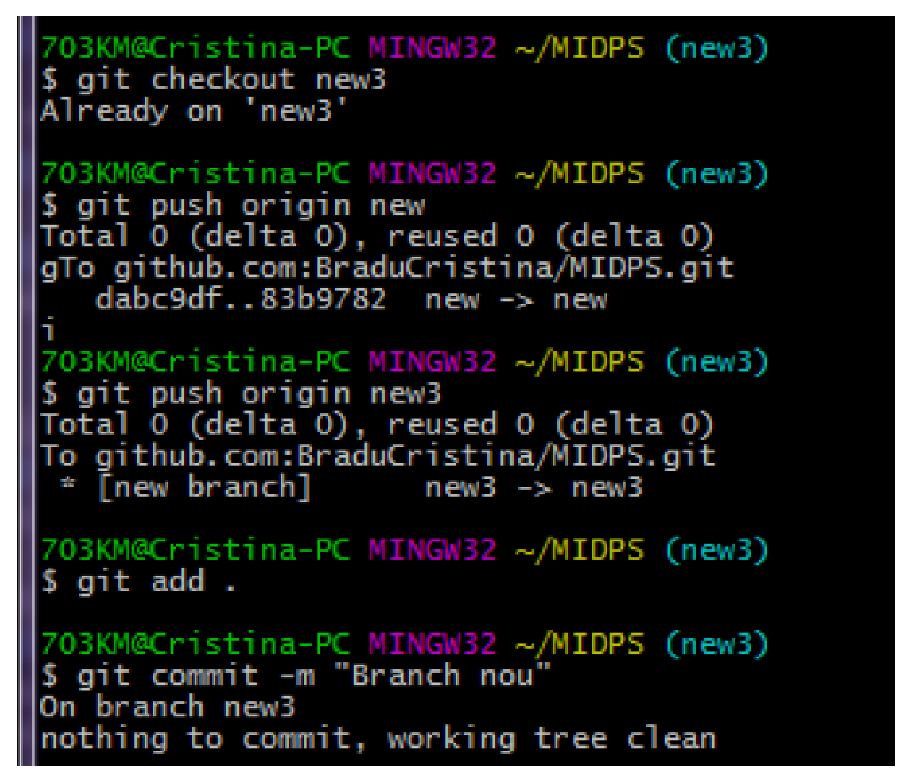
\includegraphics{images/16.eps}
\caption{Crearea si lucrul cu branch-urile}
\end{figure}

\begin{figure}[h]
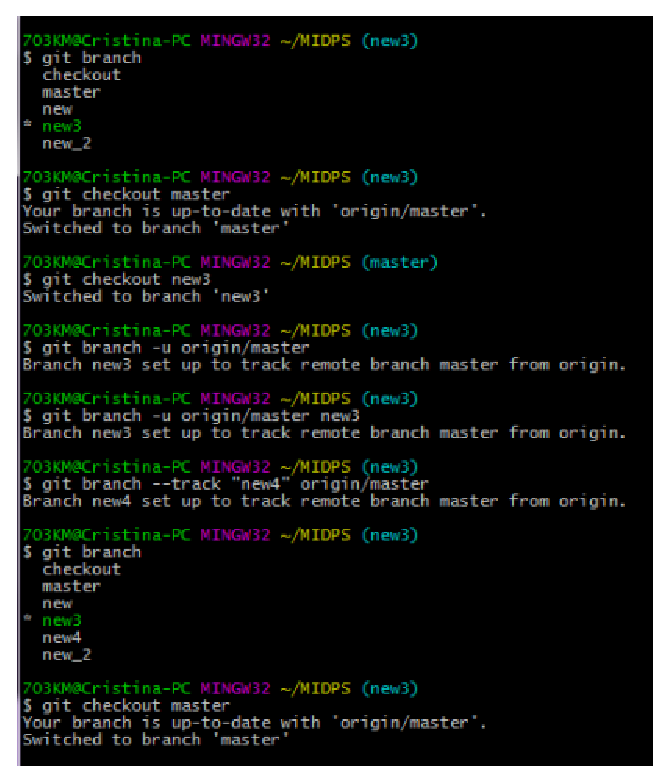
\includegraphics{images/17.eps}
\end{figure}

\begin{figure}[h]
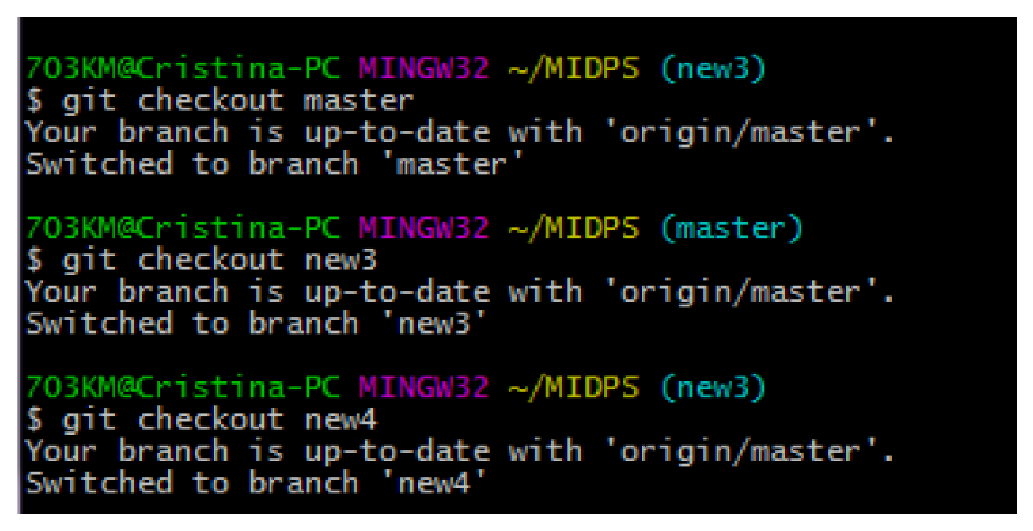
\includegraphics{images/18.eps}
\caption{Crearea si lucrul cu tracking}
\end{figure}


\begin{figure}[h]
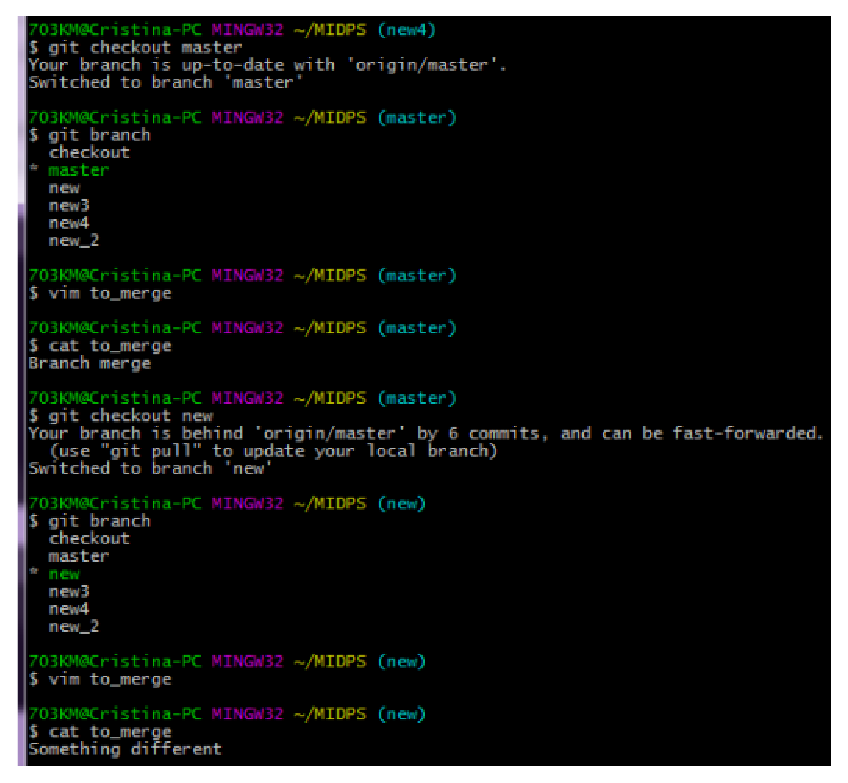
\includegraphics{images/19.eps}
\caption{Crearea fisierului tomerge}
\end{figure}

\begin{figure}[h]
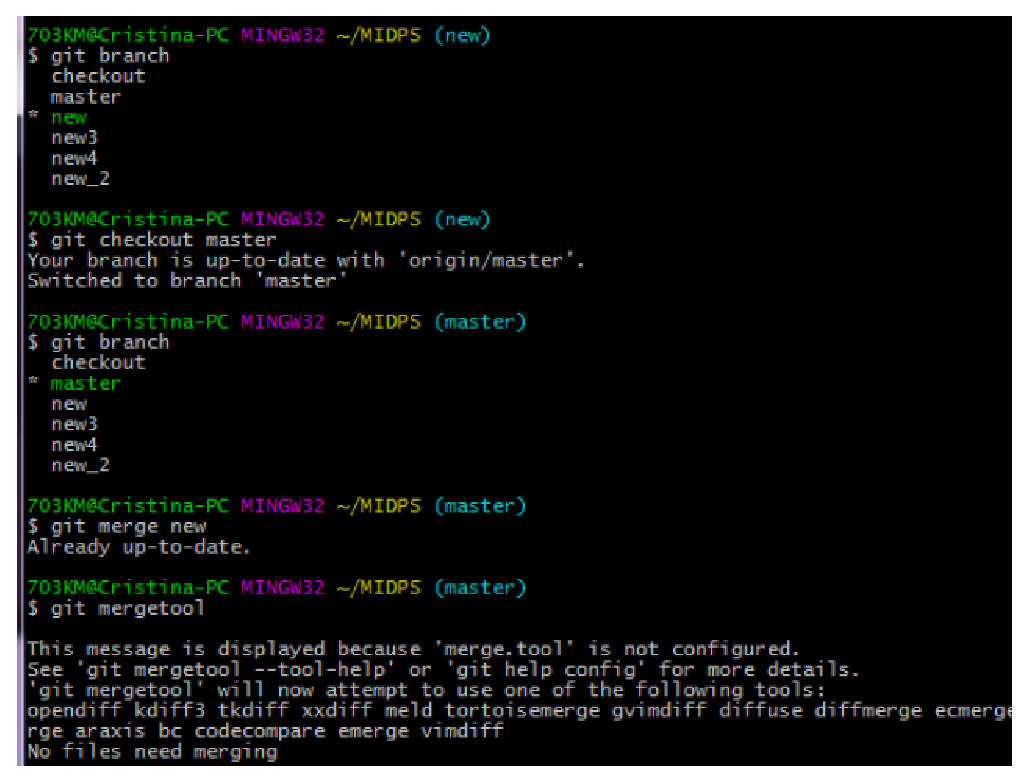
\includegraphics{images/20.eps}
\end{figure}

\begin{figure}[h]
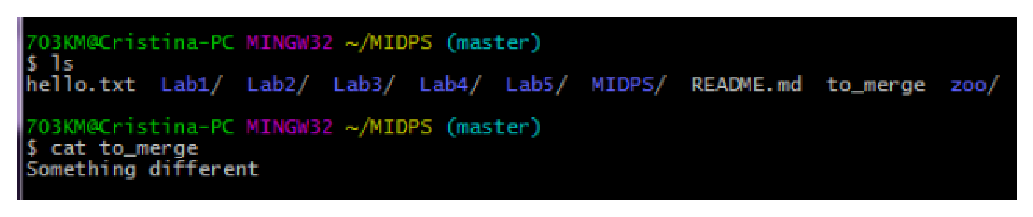
\includegraphics{images/21.eps}
\caption{Rezolvarea conflictului}
\end{figure}
%------------------------------------------------------------

\clearpage
\section*{Concluzie}

In lucrarea de laborator nr.1 la disciplina MIDPS, am facut cunostinta
cu VCS(Version Control System). VCS reprezinta niste tool-uri software,
care usureaza lucrul in echipa asupra unui proiect propus.
Gratie VCS, echipa data isi poate organiza modificarile efectuate in cod
in orice moment. Acesta salveaza track-urile modificarilor, astfel, sistemul dat
devenind destul de eficient si ofera posibilitatea de a lucra in paralel asupra
unui proiect intr-un timp mult mai scurt.
Revenirea la o versiune mai veche la fel este un avantaj al VCS.
Pentru a indeplini lucrarea de laborator, am atins asa obiective, ca crearea fisierelor,
editarea lor, crearea ramurilor si rezolvarea conflictelor aparute. Efectuarea commit-urilor
la fel a fost un punct care urma sa-l implementez, ceea ce am si reusit sa fac.
Toate comenzile care le-am utilizat, le-am indeplinit pe Windows 7.

\clearpage

\end{document}